\chapter{ОПИСАНИЕ ВЫБОРКИ}

В качестве объектов исследования выступают файлы сложного формата \textbf{doc}.
Данный вид файлов используется для хранения текстовой и графической информации, а основным программным продуктом, позволяющим их создавать и редактировать, является Microsoft Word.
Документы данного формата внутри имеют бинарную структуру, схожую по строению со структурой файловых систем. \cite{doc_format}

Как было сказано, основной задачей данной работы является описание и построение алгоритма, способного самостоятельно и в автоматическом режиме определять степень вредоносности файлов формата \textbf{doc}.
Для достижения данной цели мы будем использовать комбинацию известных алгоритмов, позволяющих учитывать предыдущий опыт -- так называемых обучаемых алгоритмов.
В нашем случае под предыдущим опытом стоит понимать наличие информации о двух наборах файлов: множество безопасных для работы документов и множество вредоносных документов.
Объеденение этих двух наборов мы в дальнейшем будем называть выборкой объектов, подразумевая что файлы были получены из некоторого нам неизвестного распределения всех возможных файлов формата \textbf{doc}. 
Процесс получения данных наборов называется разметкой и почти всегда данный процесс происходит в ручном режиме.
Тем не менее обычно нас не интересуют каким способом было получено разделение файлов на разные типы, но при этом для нас очень важно, что вероятность ошибочного размещение документа в не подходящем классе была близка к нулю, иначе, основываясь на плохо размеченной выборке объектов, мы можем создать ошибочную модель, допускающую при работе заметное число ошибок.

В отличие от ручного анализа, когда все действия, выполняемые программой при работе с документом, анализируются человеком, нам для успешного создания работающей модели важно наличие файлов различных типов.
Таким образом, в качестве первого шага, мы опишем состав нашей выборки объектов, информацию о которых в дальнейшем будем использовать как исходные данные для алгоритмов обучения.

\section{Вредоносные файлы}

На данный момент известно огромное множество видов вредоносных программ.
Также существуют различные формальные классификации, позволяющие присвоить метку почти любому вредоносному объекту: от игрушечных программ-шуток до целенаправленного высокотехнологичного программного оружия.

Под вредоносной программой принято подразумевать файл исполняемого формата, например \textbf{exe}, при запуске которого управление получает код, выполняющий несанкционированные действия относительно пользователя или владельца компьютера. 
Данный способ, захватывающий поток исполнения, довольно надёжен, но при этом имеет весьма существенный и неустранимый недостаток -- пользователь должен собственноручно инициировать начало исполнения кода.
Также такой сценарий захвата через исполняемый файл хорошо изучен в мире, что уменьшает шансы успешного прохождения возможного барьера из современных антивирусов.
В нашем случае объектом исследования являются файлы формата \textbf{doc}, предназначенные для хранения и отображения текстовой информации. 
Ожидаемым поведением при открытии файла такого формата является отображение текста, но никак не запуск произвольного и некотролируемого программного кода.
Данный факт значительно увеличивает процент людей, которые будут успешно атакованы.

Главной причиной, дающей возможность злоумышнику исполнять произвольный код при работе с неисполняемыми объектами, являются ошибки, допущенные при написании исходного кода программ, непосредственно взаимодействующих с пользовательскими файлами. 
Для объектов формата \textbf{doc} существует несколько таких программ.
Мы будем исследовать только работу Microsoft Word.
С момента первого выпуска данного текстового процессора были найдены десятки подобных ошибок, чем успешно пользуются многие авторы вирусов.
Одной из таких ошибок, например, является недостаточная или неполная проверка данных, вводимимых пользователем тем или иным способом через документ.
Забытая проверка на максимальную длину для введённой строковой последовательности выливается в размещение данных в блоке памяти, имеющем меньшей размер, чем необходимо. 
Таким образом, ввиду особенностей организации хранения служебной информации в современном компьютере, злоумышленник получает возможность видоизменять их и в итоге влиять на поток исполнения исходной программы.
Данная техника называется атакой на переполнение буфера и широко применяется в сфере компьютерной безопасности.

Работу такого вида вирусов можно разделить на следующие этапы:

\begin{itemize}
\item эксплуатирование ошибки
\item работа промежуточного машинного кода
\item работа основной функциональности вируса
\end{itemize}

В виду ограничений, возникающих во время использования уязвимости, очень редко удаётся выполнить необходимые действия сразу же после перехода на программный код злоумышленника.
Поэтому после эксплуатация ошибки управление получает промежуточный машинный код, именуемый шелл-кодом.
Задачей шелл-кода является подготовка пользовательского окружения для запуска основной функциональности вируса.
В основном промежуточный код либо производит распаковку дополнительных данных из \textbf{doc} файла, либо скачивает основную часть функциональности вируса через локальную или глобальную сеть.
Таким образом шелл-код предоставляет модульность работы вредоносного кода, то есть работа промежуточного кода и работа основного кода может быть не связана.
Более того, каждый из этих этапов зачастую реализован разными людьми.

В исследуемую выборку были отобранны файлы, работающие описанным выше образом.
Процесс формирования такого набора объектов занял продолжительное время, так как в основном осуществлялся в ручном режиме.
Также обязательным условием была полная работоспособность файла в лабораторных условиях.

Мною было произведено дизассемблирование вирусных программ, с целью более подробного изучения работы шелл-кода после эксплуатирования уязвимостей.

\newpage
\subsection{Обзор работы шелл-кода №1}

В рассмотренном примере шелл-код получает управление после использования ошибки в обработке таблицы шрифтов.
Её структура отображена на рисунке 1.1. 

\begin{figure}[ht]
	\centering
    \begin{subfigure}[b]{1\textwidth}
    \centering
        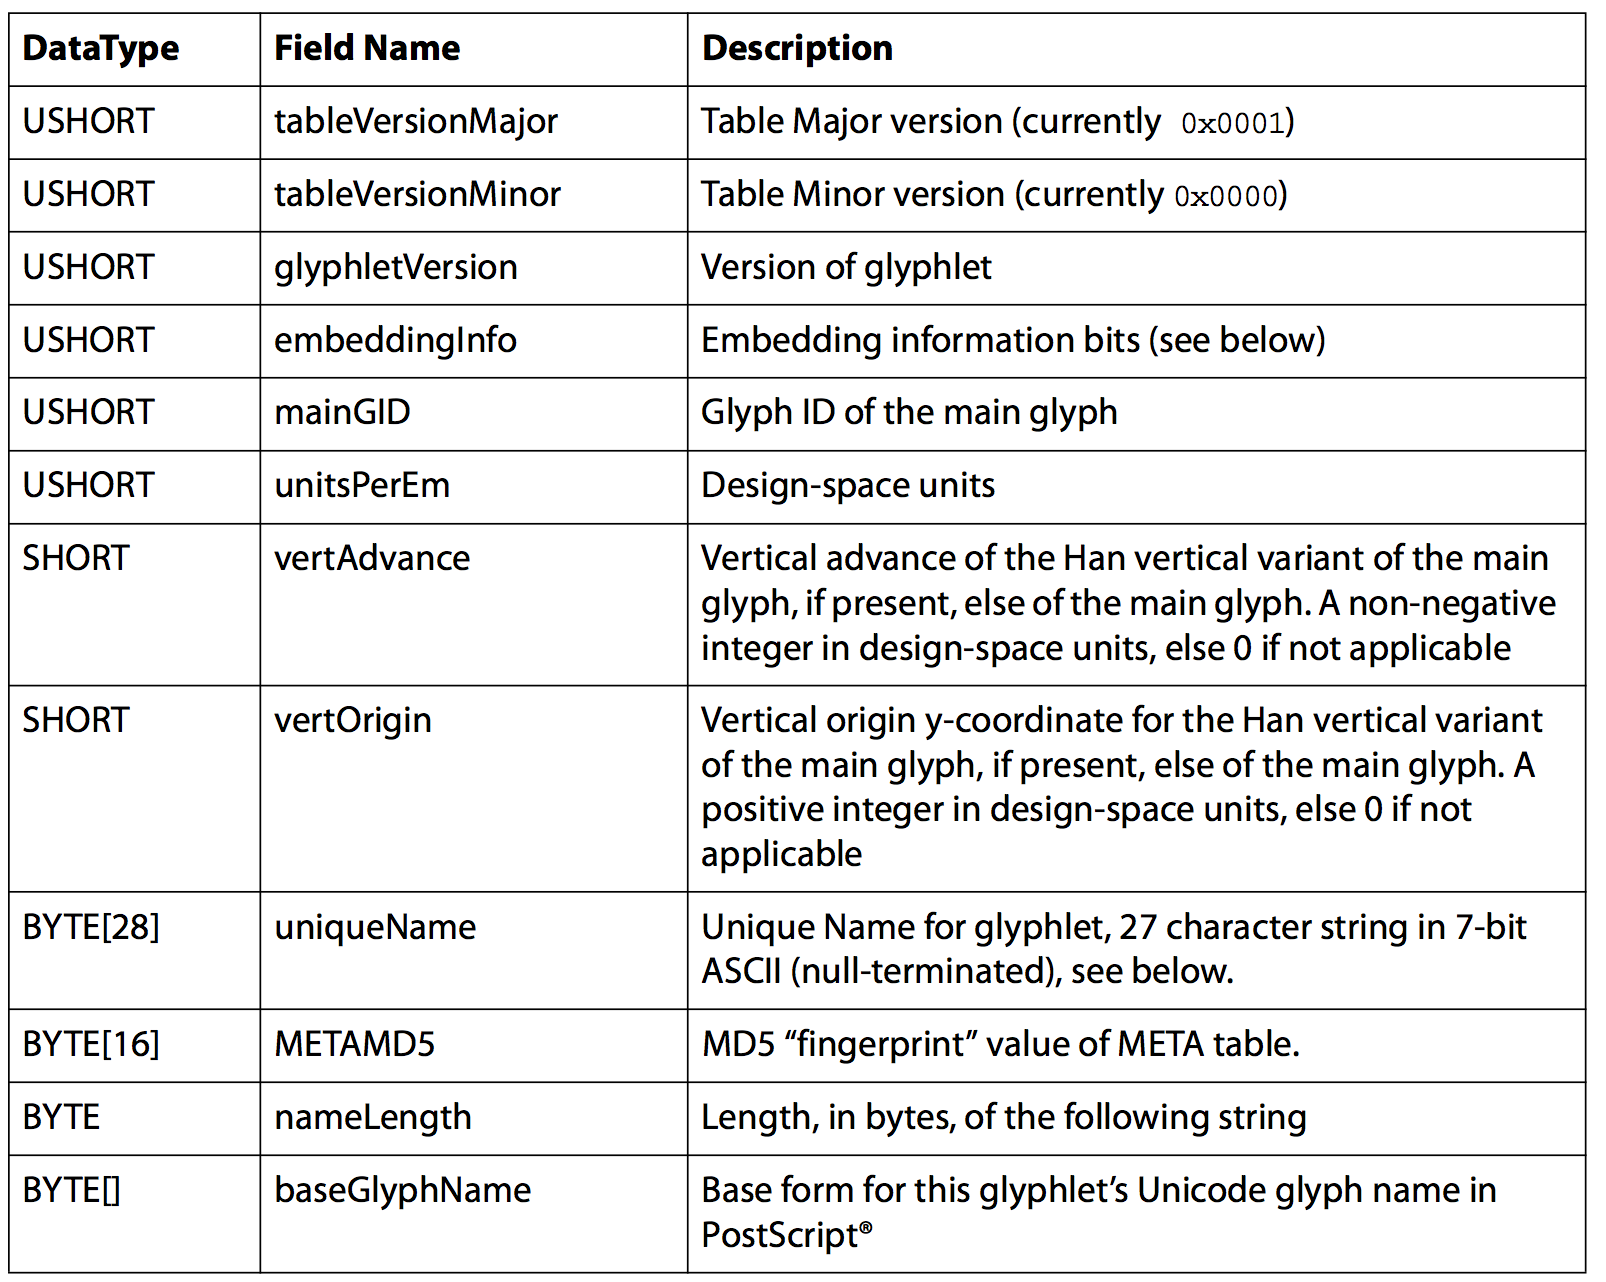
\includegraphics[scale=0.5]{1.pdf/pasted-image-15.png}
    \end{subfigure}
 
    \caption{Формат таблицы шрифтов SING}
    \label{fig_parsetree}
\end{figure}

Как можно видеть из рисунка на поле с названием \textbf{uniqueName} отводится ровно 28 байт, включаю конечный нулевой байт.
Из-за забытой проверки на длину данного поля, мы можем передавать произвольной длины названия шрифтов и изменять адрес возврата функции.

С помощью технологии HeapSpray память процесса наполняется 


\subsection{Обзор уязвимости для формата doc}



\section{Безопасные файлы}

Чтобы построенная модель могла определять степень вредоносности объектов, ей при построении необходимо в дополнение к информации, полученной по вредоносным файлам, подать на вход данные, собранные по безвредным объектам.
В отличие от вредоносных объектов, безвредные объекты могут быть созданы непосредственно с помощью текстового редактора Microsoft Word.
Так как выборка должна иметь конечный размер, нам необходимо ограничить набор безвредных файлов, которые попадут в исходные данные для обучения.
При этом нам нужно добиться разнообразия среди файлов.

Основной идеей было выделение основных характеристик документа и объединения их значений в различных комбинациях.
В качестве таких характеристик были использованы следующие позиции:
\begin{itemize}
\item количество страниц
\item вариант используемого шрифта
\item наличие таблиц
\item наличие встроенной графики
\item наличие графических изображений
\item использование нестандартных стилей
\item визуальное форматирование текста
\end{itemize}

Перечисленный набор характеристик представляется достаточным для построения выборки разнообразных безопасных файлов и был принят в качестве отправной точки.
Анализ результатов работы, а так же более подробный обзор функционала программного обеспечения Microsoft Word и дальнейшая кластеризация характеристик безопасных файлов могут повысить качество создаваемой модели.
Для сохранения баланса между безвредными и вредоносными файлами было создано 15 безопасных объектов.